\documentclass[sigconf,screen,review,balance=false]{acmart}

\usepackage{subcaption}
\usepackage{lmodern}

\let\Bbbk\relax

\usepackage{xcolor}
\usepackage{enumitem}
\usepackage{color}
\usepackage{adjustbox}
\usepackage{array}
\usepackage{tabularx}
\usepackage{xspace}
\usepackage[strings]{underscore}
\usepackage{nicematrix}
\usepackage{amssymb}
\usepackage{microtype}
\usepackage[normalem]{ulem}
\usepackage{graphicx}
\usepackage{booktabs}
\usepackage{svg}
\usepackage{bbding}
\usepackage[dvipsnames]{xcolor}
\definecolor{redish}{RGB}{221, 42, 43}
\usepackage{pifont}
\usepackage{hyperref}

\usepackage[most]{tcolorbox}
\usepackage{algorithm}
\usepackage{algpseudocode}
\usepackage{amsmath}
\usepackage{amsfonts}
\usepackage{bm}
\usepackage{listings}
\usepackage{lstautogobble}
\usepackage{tikz}
\usepackage{pict2e}
\usepackage{multirow}
\usepackage{mathtools}
\usepackage{mdframed}
\usepackage{syntax}
\usepackage{colortbl}
\usepackage{tikz-qtree}

% Defined colors
\definecolor{add-line}{rgb}{0.84, 0.89, 0.97}
\definecolor{add-word}{rgb}{0.5, 0.7, 0.98}
\definecolor{ForestGreen}{RGB}{63,147,88}
\definecolor{remove-line}{rgb}{1.0, 0.93, 0.73}
\definecolor{remove-word}{rgb}{1.0, 0.8, 0.2}
\definecolor{Gray}{gray}{0.9}
\definecolor{orange}{rgb}{0.84, 0.89, 0.89}

% Theorem environments
\newtheorem{definition}{Definition}[section]
\newtheorem{theorem}{Theorem}[section]
\newtheorem{corollary}{Corollary}[section]

% Custom commands
\newcommand{\hlcode}[1]{\colorbox{yellow}{\ttfamily #1}}
\newcommand{\tabincell}[2]{\begin{tabular}{@{}#1@{}}#2\end{tabular}}
\newcommand{\redout}{\bgroup\markoverwith{\textcolor{red}{\rule[.45ex]{1.5pt}{1.pt}}}\ULon}

\newcommand\Myperm[2][^n]{\prescript{#1\mkern-2.5mu}{}P_{#2}}
\newcommand\Mycomb[2][^n]{\prescript{#1\mkern-0.5mu}{}C_{#2}}

% Algorithm-related
\algnewcommand{\LineComment}[1]{\Statex #1}
\algrenewcommand\algorithmicindent{1.0em}
\algdef{SE}[DOWHILE]{Do}{doWhile}{\algorithmicdo}[1]{\algorithmicwhile\ #1}

% Math operators
\DeclareMathOperator*{\argmax}{argmax}
\DeclareMathOperator*{\argmin}{argmin}

% TikZ libraries
\usetikzlibrary{shapes,positioning,arrows.meta, calc, decorations.pathreplacing, matrix}

% Code listing style
\lstdefinestyle{mystyle}{
    frame=single,
    framexleftmargin=0pt,
    commentstyle=\color{ForestGreen},
    keywordstyle=\color{blue}\bfseries,
    numberstyle=\normalsize\color{gray},
    stringstyle=\color{purple},
    basicstyle=\scriptsize\ttfamily\bfseries,
    breakatwhitespace=false,
    breaklines=false,
    captionpos=b,
    keepspaces=true,
    numbers=none,
    numbersep=4pt,
    showspaces=false,
    showstringspaces=false,
    showtabs=false,
    tabsize=2,
    language=C++,
    escapechar=\@,
    moredelim=**[is][{\btHL[fill=red!40]}]{@}{@},
    moredelim=**[is][{\btHL[fill=remove-line]}]{|*}{*|},
    moredelim=**[is][{\btHL[fill=remove-word]}]{|^}{^|},
    moredelim=**[is][{\btHL[fill=add-line]}]{||^}{^||},
    moredelim=**[is][{\btHL[fill=add-word]}]{||*}{*||}
}

\lstdefinestyle{inlinestyle}{
    language=C++,
    basicstyle=\small\ttfamily\bfseries,
}

% tcolorbox environments
\newtcolorbox{findingbox}[1]{
    colback=red!5!yellow!10!white,
    colframe=red!50!black,
    sharp corners,
    boxrule=0.6pt,
    fontupper=\itshape,
    enhanced,
    before upper={\textbf{\textcolor{red!50!black}{Finding #1.}}~}
}

\global\mdfdefinestyle{default}{
    usetwoside=false,
    linecolor=black,linewidth=1pt,
    innerleftmargin=5pt,innerrightmargin=5,
    everyline=true
}

\newcommand{\lstbg}[3][0pt]{{\fboxsep#1\colorbox{#2}{\strut #3}}}
\newcommand{\circled}[1]{\tikz[baseline=(char.base)]{\node[shape=circle,draw,inner sep=0.1pt] (char) {#1};}}

% Font commands
\newcommand{\textmtte}[1]{{\fontsize{9}{11}\fontfamily{txtt}\selectfont #1}}
\renewcommand{\texttt}[1]{\textmtte{#1}}
\newcommand{\myinline}{\lstinline[style=inlinestyle]}
\newcommand{\myparagraph}[1]{\vspace{3pt}\textbf{\textit{#1}}\,}
\newcommand{\todocite}{{\color{magenta} \sf [?]}}

% Highlight environment
\makeatletter
\newenvironment{btHighlight}[1][]
{\begingroup\tikzset{bt@Highlight@par/.style={#1}}\begin{lrbox}{\@tempboxa}}
{\end{lrbox}\bt@HL@box[bt@Highlight@par]{\@tempboxa}\endgroup}

\newcommand\btHL[1][]{
    \begin{btHighlight}[#1]\bgroup\aftergroup\bt@HL@endenv%
}
\def\bt@HL@endenv{
    \end{btHighlight}%
    \egroup
}
\newcommand{\bt@HL@box}[2][]{
    \tikz[#1]{
        \pgfpathrectangle{\pgfpoint{1pt}{0pt}}{\pgfpoint{\wd #2}{\ht #2}}
        \pgfusepath{use as bounding box}
        \node[anchor=base west, fill=orange!25,outer sep=.5pt,inner xsep=0.5pt, inner ysep=0.15pt, rounded corners=1pt, minimum height=\ht\strutbox-.1pt,#1]{\raisebox{.01pt}{\strut}\strut\usebox{#2}};
    }%
}
\makeatother

\newcommand{\cf}{\hbox{\emph{cf.}}\xspace}
\newcommand{\etal}{\hbox{et al.}\xspace}
\newcommand{\eg}{\hbox{\emph{e.g.}}\xspace}
\newcommand{\ie}{\hbox{\emph{i.e.}}\xspace}
\newcommand{\st}{\hbox{\emph{s.t.}}\xspace}
\newcommand{\wrt}{\hbox{\emph{w.r.t.}}\xspace}
\newcommand{\etc}{\hbox{\emph{etc.}}\xspace}
\newcommand{\resp}{\hbox{\emph{resp.}}\xspace}
\newcommand{\defa}{\hbox{\emph{de facto}}\xspace}
\newcommand{\vice}{\hbox{vice versa}\xspace}

%% Rights management information.
%% Remove or fill in with actual values for camera-ready.
\setcopyright{acmcopyright}
\copyrightyear{2026}
\acmYear{2026}
\acmConference[ICSE '27]{The 49th International Conference on Software Engineering}{April 2027}{Rio de Janeiro, Brazil}

%% Submission ID (uncomment when available).
%% \acmSubmissionID{123-A56-BU3}

%% Citation style.
\citestyle{acmnumeric}

%% Tool name.
\newcommand{\tool}{\textsf{CodeArena}\xspace}

%% Author comment macros (hidden in the submitted version).
\newcommand{\wyc}[1]{}
\newcommand{\hzbc}[1]{}
\newcommand{\todo}[1]{}

\title[\tool]{\tool: A Dynamic Benchmarking Framework for Trustworthy Evaluation of Code-Generation Models}

\author{Anonymous Author(s)}
\affiliation{
  \institution{Anonymous Institution}
  \country{Anonymous Country}
}
\email{anonymous@example.com}

\begin{document}

\begin{abstract}
The rapid progress of large-scale code generation models has intensified the need for trustworthy benchmarks. Existing static benchmarks are increasingly vulnerable to data contamination, because their tasks and canonical solutions can be absorbed into training corpora, inflating reported accuracy without reflecting genuine reasoning ability. We introduce \tool{}, an LLM-driven dynamic benchmarking framework that alleviates this problem by automatically mutating seed programming tasks into semantically related yet functionally distinct variants. Given an existing benchmark task, \tool{} prompts an \emph{Attacker} model to refactor the canonical solution, constructs a new task statement grounded in executable test cases, and then evaluates a set of \emph{Defender} models on the mutated tasks. The resulting adversarial setup provides a moving target for data-contaminated models while remaining fair to models that generalize. We further derive an Elo-based holistic rating that consolidates both the problem-solving and problem-generation abilities of each model. Experiments on HumanEval and Codeforces-derived tasks show that \tool{} substantially reduces the performance inflation caused by fine-tuning on leaked data and produces evaluation scores that correlate far more closely with a model's uncontaminated capability than prior static or perturbation-based baselines.

\end{abstract}

\keywords{large language models, code generation, benchmark, data contamination, trustworthy evaluation}

\begin{CCSXML}
<ccs2012>
   <concept>
       <concept_id>10011007.10011074.10011099.10011105.10011114</concept_id>
       <concept_desc>Software and its engineering~Software verification and validation</concept_desc>
       <concept_significance>500</concept_significance>
   </concept>
   <concept>
       <concept_id>10010147.10010178.10010179.10010182</concept_id>
       <concept_desc>Computing methodologies~Natural language generation</concept_desc>
       <concept_significance>300</concept_significance>
   </concept>
   <concept>
       <concept_id>10011007.10011074.10011784</concept_id>
       <concept_desc>Software and its engineering~Search-based software engineering</concept_desc>
       <concept_significance>300</concept_significance>
   </concept>
</ccs2012>
\end{CCSXML}

\ccsdesc[500]{Software and its engineering~Software verification and validation}
\ccsdesc[300]{Computing methodologies~Natural language generation}
\ccsdesc[300]{Software and its engineering~Search-based software engineering}

\maketitle


\section{Introduction}

The rapid advancement of large-scale code generation models (LCGMs) has enabled them to address a broad range of general programming tasks~\cite{chen2021evaluating, openai2023gpt4, team2023gemini, touvron2023llama2}. Although these advances are promising, they also raise critical concerns regarding performance evaluation. A benchmark that enables accurate and objective assessment is indispensable for both users and developers. Consequently, numerous benchmarks have been introduced~\cite{chen2021evaluating, jain2024livecodebench, zhuo2024bigcodebench}, most of which rely on static, ground-truth-based evaluation.

\subsection{Data Contamination}

``When a measure becomes a target, it ceases to be a good measure.'' Achieving trustworthy evaluation is challenging. One of the most significant obstacles is \emph{data contamination}, which arises when test data is included in a model's training set, leading to an overestimation of its true performance. Because of this inflation, the observed gains do not generalize to real-world programming tasks, the benchmark's utility declines, and developers lose confidence in the reported numbers. In effect, every static benchmark has a finite useful lifetime.

Manually refreshing static benchmarks is an insufficient remedy for data contamination. The problem is rooted in the static and open-source nature of contemporary benchmarks, which allows evaluation tasks to be readily incorporated into training corpora, thereby artificially inflating accuracy metrics~\cite{yang2023rethinking}. Rebuilding a benchmark from scratch is straightforward in principle, but problematic in practice. First, designing and disseminating a new benchmark---especially one that targets a specialized domain---requires substantial time and human effort. Second, although frequent benchmark updates seek to mitigate this risk, the pace of contamination often exceeds the multi-month cycles required for formal benchmark releases. Consequently, the rapid fine-tuning of models---often completed within days---can render newly released datasets such as KernelBench~\cite{lange2025robustagenticcudakernel} or historical problems in LiveCodeBench~\cite{jain2024livecodebench} obsolete almost immediately. Therefore, manual updates to static benchmarks cannot adequately address data contamination.
To tackle this issue, existing research has explored two primary directions. The first direction is \emph{task perturbation}, which translates, rewrites, adapts, or merges existing benchmark tasks so that the updated tasks differ from the data seen during training. The second direction is \emph{contamination detection}, which uses predefined features to detect whether a model has been contaminated by a benchmark; some methods even leverage detection results to mitigate the contamination.

\subsection{Limitations of Existing Methods}

Both directions exhibit fundamental limitations. First, traditional task-generation and perturbation methods often fail to produce sufficiently challenging tasks. Approaches such as RECODE~\cite{wang-etal-2023-recode} primarily perturb task descriptions while leaving canonical solutions unchanged and therefore retrievable from model parameters. Although PPM~\cite{10.1145/3643780} transforms code outputs, these variants are often too simplistic for modern LCGMs. More importantly, current generation methods---such as sequentially combining independent problems into a single task---are easily decomposed and solved by advanced models. Ultimately, creating complex, diverse, and verified task variants still requires substantial manual effort to ensure the correctness of test cases, thereby lacking the scalability necessary for rapid iteration of LLMs.

Second, methods based on contamination detection are constrained by inaccurate leakage patterns and limited applicability. Many effective detection techniques~\cite{nguyen2025rn} require access to internal model parameters or log-probabilities, which renders them inapplicable to widely used closed-source LLMs such as GPT, Claude, and Gemini. Even in output-based detection, methods that measure similarity across multiple outputs~\cite{dong-etal-2024-generalization} frequently yield false positives. The fundamental flaw in this reasoning is that, for simple but fundamental problems, nearly all correct solutions are inherently similar; incorrectly flagging these as leaked results in a biased and ineffective evaluation of a model's true capability. More importantly, most contamination detection methods cannot be directly applied to reliability assessment because they cannot determine how the model actually performs on test sets that have not been leaked.

\subsection{Our Approach}

To address these limitations, we introduce \tool{}, an automated pipeline for adapting programming tasks. Inspired by the ability of models to solve concrete problems, we hypothesize that they can also adapt problems with high quality. We exploit this capability to design a fully automated pipeline. First, we provide a model with the canonical solution of a programming task and pose an open-ended refactoring request, asking the model to modify the code's functionality. Next, we construct a code-generation prompt for the mutated code, including the problem description and test cases, thereby forming a new, self-contained programming task. Finally, the pipeline equips the task with the corresponding test harness. In the following sections, we discuss how our method mitigates data contamination and empirically demonstrate its effectiveness.

\myparagraph{A High-Level Approach to Our Evaluation.} The objective of our method is to achieve automated evaluation while mitigating contamination. We follow the idea of task- generation based methods, but realize it by leveraging LLMs. First, we formulate an open-ended question that prompts models to mutate code selected from the current benchmark in order to transform its functionality. Then, we construct a novel programming task, which primarily comprises the prompt that guides the model to generate the target code and the test code based on the mutated code, and we use it to evaluate the current model. We repeat the above procedure several times and finally calculate each model's score from its answers and the quality of the mutated code.


\hzbc{Put challenge here better or 2.1???    Here I will supply the criteria the quality of the mutated task }
It is clear that the main challenge lies in the first step---how can we ensure that the mutated task is able to mitigate data contamination? One straightforward approach would be to ask the model to generate a program together with the problem statement and test cases directly. However, this would raise several issues: the generated test cases may be inconsistent with the code, the problem description may be ambiguous, and the resulting tasks may be either too easy or computationally infeasible. Instead, we pursue an alternative route: we mutate an existing verified solution and derive the new task and test cases directly from the mutated code. This guarantees consistency and tractability by construction.

\label{sec:intro}

\section{Methodology}

In this section, we present a high-level workflow of our approach. 

\subsection{Workflow}
\begin{figure}[t!]
	\captionsetup{skip=5pt}
	\centering
	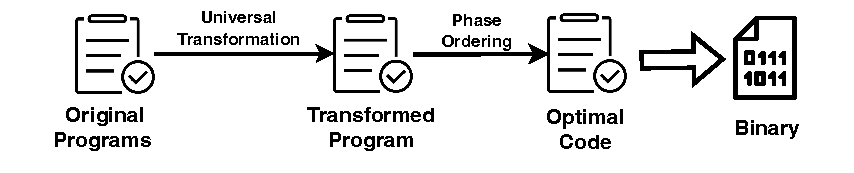
\includegraphics[width=\textwidth]{pics/workflow.pdf}
	\caption{\tool's workflow.}
	\label{fig:keycom}
\end{figure}

\subsection{bbb}

\section{Experiment}
\label{sec:experiment}

\subsection{Research Questions}

We focus on the following research questions:

\textbf{RQ1 (Effectiveness):} To what extent can AI-generated tasks effectively mitigate the impact of data contamination and facilitate a more trustworthy evaluation of large language models?

\textbf{RQ2 (Attacker vs.~Defender ability):} How differently does an LLM perform in our open-ended code-refactoring generation tasks compared with its performance in well-defined, specific problem-solving tasks?

\textbf{RQ3 (Estimation error):} What is the estimation error of our method relative to the uncontaminated baseline?

\textbf{RQ4 (Cost):} What is the computational and monetary cost of running \tool{}?

\subsection{Single-Task Analysis for Fine-Tuned Models}

Previous studies have often focused on evaluating fluctuations in overall benchmark metrics while lacking fine-grained analysis of individual tasks. This makes it difficult to determine whether performance degradation genuinely stems from effective interception of data leaks, primarily because tracing where models are contaminated across specific tasks is challenging. To address this, we construct a more causally explicit experimental environment by simulating data leaks and adversarial scenarios at their source, significantly enhancing the reliability of evaluation results.

\begin{table*}[th!]
\centering
\caption{Comparison between \tool{} and other contamination-detection approaches.}
\label{table3}
\resizebox{\textwidth}{!}{%
\begin{tabular}{@{}lcccccc@{}}
\toprule
Approach & No Manual Rules & No New Benchmark & No Extensive Sampling & Easy to Expand & Scalable & Dynamic \\
\midrule
PPM ~\cite{chen2024ppm}   &
$\times$ & $\times$ & $\checkmark$ & $\times$ & -- & -- \\
CDD / TED ~\cite{dong-etal-2024-generalization}  &
$\checkmark$ & $\times$ & $\times$ & $\times$ & -- & -- \\
\tool{} &
$\checkmark$ & $\checkmark$ & $\checkmark$ & $\checkmark$ & $\checkmark$ & $\checkmark$ \\
\bottomrule
\end{tabular}
}
\end{table*}

\textbf{Experimental Setup.} We employ fine-tuning techniques to simulate data-leakage scenarios. Given the high computational cost of full-parameter fine-tuning, we selected models with parameter ranges between 7 billion and 32 billion as defenders. These models are specifically designed for code-generation tasks in on-premises deployment scenarios. Through targeted fine-tuning, we can precisely identify the actual data causing contamination and its severity. Concurrently, we utilize API calls to full-parameter models as attackers. We compare \tool{} with the following baselines: (1) \textbf{PPM}~\cite{chen2024ppm}; (2) \textbf{TED}~\cite{dong-etal-2024-generalization}; (3) \textbf{AutoCode}; and (4) additional baselines to be added in the final version.

\textbf{Data Preparation.} The datasets used for fine-tuning were collected from Codeforces from 2022 to 2025. For each year, we gathered 50 tasks with Python solutions. We did not use well-known benchmarks such as HumanEval for fine-tuning because the fine-tuned model could not outperform the original model, even when trained for a wide range of epochs. This suggests that those benchmarks may already have been subject to substantial data leakage.

\myparagraph{Metrics}

\textbf{1. Pass@$k$.} Pass@$k$ is the standard metric for evaluating functional correctness. Specifically, Pass@$k$ measures the probability that at least one of the top $k$ generated code samples passes a set of unit tests. Mathematically, if we generate $n$ samples for each problem and $c$ of them pass the unit tests ($c \le n$), the unbiased estimator of Pass@$k$ is defined as:
\begin{align}
\text{Pass@}k = \mathbb{E} \left[ 1 - \frac{\binom{n-c}{k}}{\binom{n}{k}} \right]
\end{align}
where $n$ is the total number of samples generated per task, $c$ is the number of correct samples that pass the test oracles, and $k$ is the number of samples considered in the evaluation (typically $k \in \{1, 10, 100\}$).

\textbf{2. Correlation.} Previous evaluation methods have merely sought to reduce a model's score on the whole benchmark, yet this does not demonstrate the method's effectiveness. To address this, we propose evaluating a method's effectiveness by calculating the correlation coefficient between the results obtained before and after model contamination using the same method. A higher correlation coefficient indicates that the method's evaluation results cause the contaminated model to perform more closely to its uncontaminated state.

Given that the model architecture and core parameters remain consistent with the pre-trained backbone during the fine-tuning process, we hypothesize that the model's output distribution should exhibit a degree of functional stability. To quantify this, we calculate the correlation of the model's pass rates at the individual-task level, thereby measuring the consistency of its performance across different problem instances. We denote the sample scores for each task as $S = \{S_1, S_2, \dots, S_n\}$ from the original model $M$, and $S' = \{S'_{1}, S'_{2}, \dots, S'_{n}\}$ from the fine-tuned model based on $M$. The correlation is calculated as follows:
\begin{align}
r_{M} &= \frac{\sum_{i=1}^{n} (S_i - \bar{S})(S'_i - \bar{S'})}{\sqrt{\sum_{i=1}^{n} (S_i - \bar{S})^2} \sqrt{\sum_{i=1}^{n} (S'_i - \bar{S'})^2}} \label{eq:correlation}
\end{align}

\textbf{RQ1 Results.} Results are shown in Table~\ref{tab:rq1Humaneval} and Figure~\ref{fig:Qwen1Comparison}.

\begin{table*}[t!]
    \centering
    \caption{The effectiveness evaluation on the HumanEval dataset.}
    \label{tab:rq1Humaneval}
    \resizebox{\linewidth}{!}{
        \begin{NiceTabular}{lccccccccc} 
        \CodeBefore
            \rowcolors{4}{}{blue!8}
        \Body
    \toprule
    \toprule
    \textbf{Methods} & \multicolumn{3}{c}{\textbf{Qwen2.5-14B-instruct}} & \multicolumn{3}{c}{\textbf{Phi4}} & \multicolumn{3}{c}{\textbf{Gemma2-27B}} \\
    \cmidrule(lr){2-4} \cmidrule(lr){5-7} \cmidrule(lr){8-10}
    & \textbf{Before} & \textbf{After} &\textbf{Correlation} & \textbf{Before} & \textbf{After} & \textbf{Correlation} &\textbf{Before} & \textbf{After} &\textbf{Correlation} \\
    \midrule
    \textbf{Base} & 0.69 & 0.77 & 0.5351 & 0.76 & 0.77 & 0.6877 & 0.70 & 0.70 & 0.9259 \\
    \textbf{PPM}       & 0.62+ & 0.62+ (-19.5\%) & - & 0.8469 & 0.8745 (+13.6\%) & - & 0.6683 & 0.6372 \textbf{(-9.0\%)} & - \\
    \textbf{TED ($\tau=2$)}  & 0.70 & 0.64 (-16.9\%) & 0.4816 (-10.0\%) & 0.8469 & 0.8669 (+12.6\%) & 0.8355 (+21.5\%) & 0.6750 & 0.6751 (-3.6\%) & 0.9535 (+3.0\%) \\
    \midrule
    \textbf{Our Tool}  & 0.58 & 0.60 \textbf{(-22.1\%)} & \textbf{0.9666 (+80.7\%)} & 0.57 & 0.58 \textbf{(-24.7\%)} & \textbf{0.9915 (+44.2\%)} & 0.64 & 0.66 (-5.7\%) & \textbf{0.9885 (+6.8\%)} \\
    \bottomrule
    \bottomrule

    \toprule
    \toprule
    \textbf{Methods} & \multicolumn{3}{c}{\textbf{Qwen3-14B}} & \multicolumn{3}{c}{\textbf{Qwen2.5-7B-Instruct}} & \multicolumn{3}{c}{\textbf{DeepSeek-coder-14B-Preview}} \\
    \cmidrule(lr){2-4} \cmidrule(lr){5-7} \cmidrule(lr){8-10}
    & \textbf{Before} & \textbf{After} &\textbf{Correlation} & \textbf{Before} & \textbf{After} &\textbf{Correlation} & \textbf{Before} & \textbf{After} &\textbf{Correlation} \\
    \midrule
    \textbf{Base} & 0.8714 & 0.9015 & 0.9502 & 0.6904 & 0.7135 & 0.8698 & 0.56 & - & - \\
    \textbf{PPM}       & 0.8385 & 0.7875 \textbf{(-12.6\%)} & - & - & - & - & - & - & - \\
    \textbf{TED ($\tau=2$)}  & 0.8633 & 0.8054 (-10.7\%) & 0.5649 (-40.5\%) & - & - & - & - & - & - \\
    \midrule
    \textbf{Our Tool}  & 0.8295 & 0.8307 (-7.9\%) & \textbf{0.9748 (+2.6\%)} & 0.4510 & 0.4587 \textbf{(-35.7\%)} & \textbf{0.9829 (+13.0\%)} & - & - & - \\
    \bottomrule
    \bottomrule

    \toprule
    \toprule
    \textbf{Methods} & \multicolumn{3}{c}{\textbf{StarCoder2-7B}} & \multicolumn{3}{c}{\textbf{Phi-3}} & \multicolumn{3}{c}{\textbf{Yi-Coder-9B}} \\
    \cmidrule(lr){2-4} \cmidrule(lr){5-7} \cmidrule(lr){8-10}
    & \textbf{Before} & \textbf{After} &\textbf{Correlation} & \textbf{Before} & \textbf{After} &\textbf{Correlation} & \textbf{Before} & \textbf{After} &\textbf{Correlation} \\
    \midrule
    \textbf{Base} & - & - & - & 0.5247 & 0.5158 & 0.9426 & 0.7471 & 0.7433 & 0.9459 \\
    \midrule
    \textbf{Our Tool}  & - & - & - & 0.3393 & 0.3489 \textbf{(-32.4\%)} & \textbf{0.9793 (+3.9\%)} & 0.5688 & 0.5622 \textbf{(-24.4\%)} & \textbf{0.9761 (+3.2\%)} \\
    \bottomrule
    \bottomrule
    \end{NiceTabular}
    }

\begin{flushleft}
The data in the table represents the model's Pass@1 score for the corresponding evaluation method; “Before” and “After” indicate whether the model has been fine-tuned. \\
\emph{Note:} Percentages in parentheses represent change relative to Base (After/Correlation). For Pass@1, negative = better (lower). For Correlation, positive = better (higher). \textbf{Bold} indicates the best performance among PPM, TED($\tau=2$), and Our Tool for each metric.
\end{flushleft}
\end{table*}
\begin{figure*}[t!]
    \centering
    \begin{subfigure}[b]{0.48\textwidth}
        \centering
        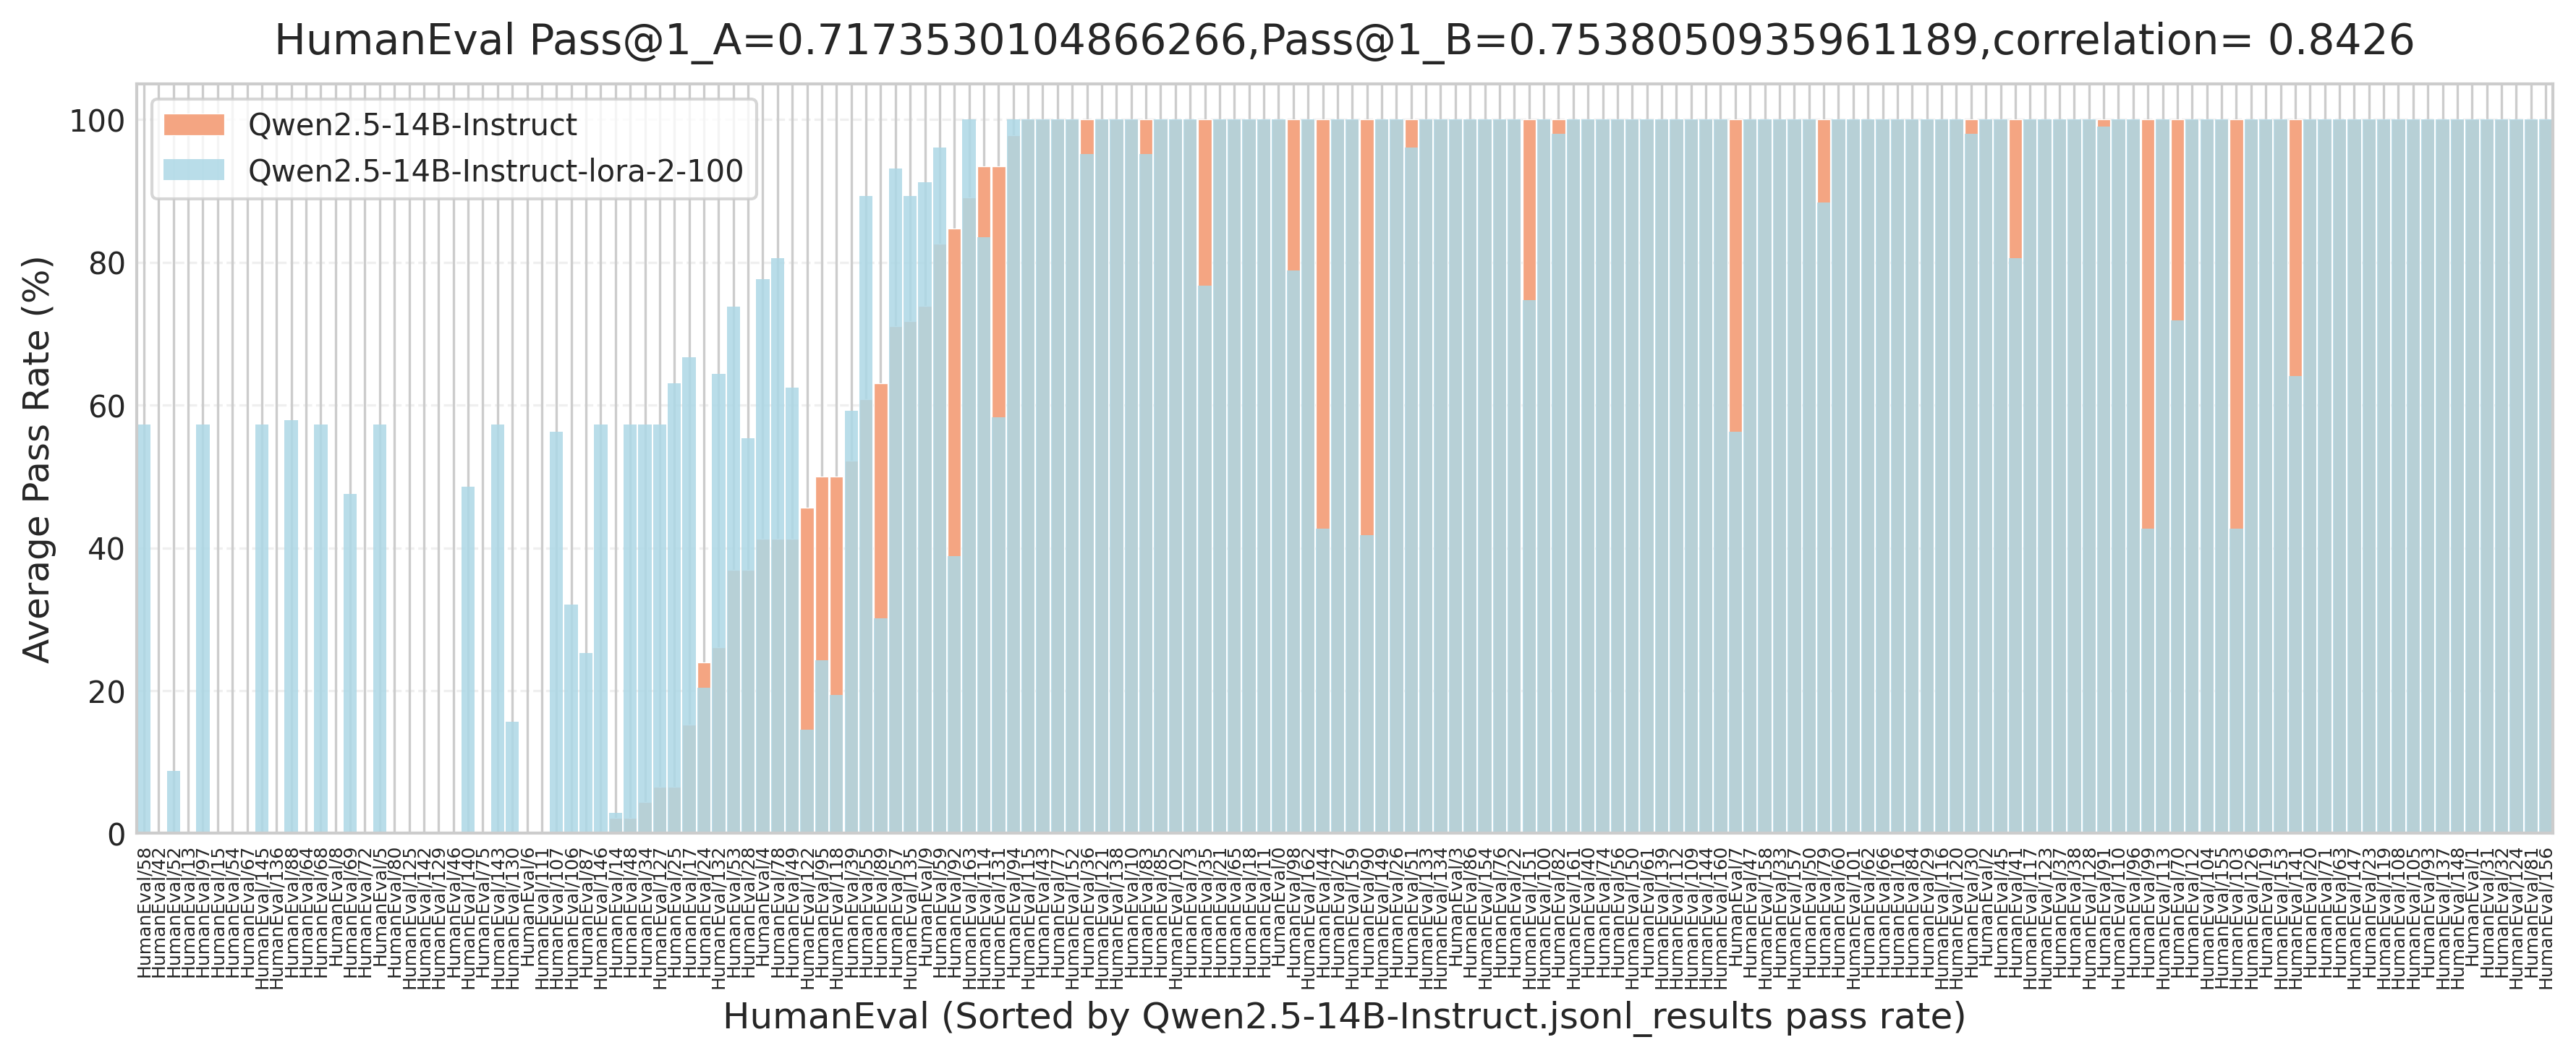
\includegraphics[width=\textwidth]{figures/Qwen.png}
        \caption{Pass@1 for Qwen2.5-14B on original HumanEval}
        \label{fig:qwensub1}
    \end{subfigure}
    \hfill
    \begin{subfigure}[b]{0.48\textwidth}
        \centering
        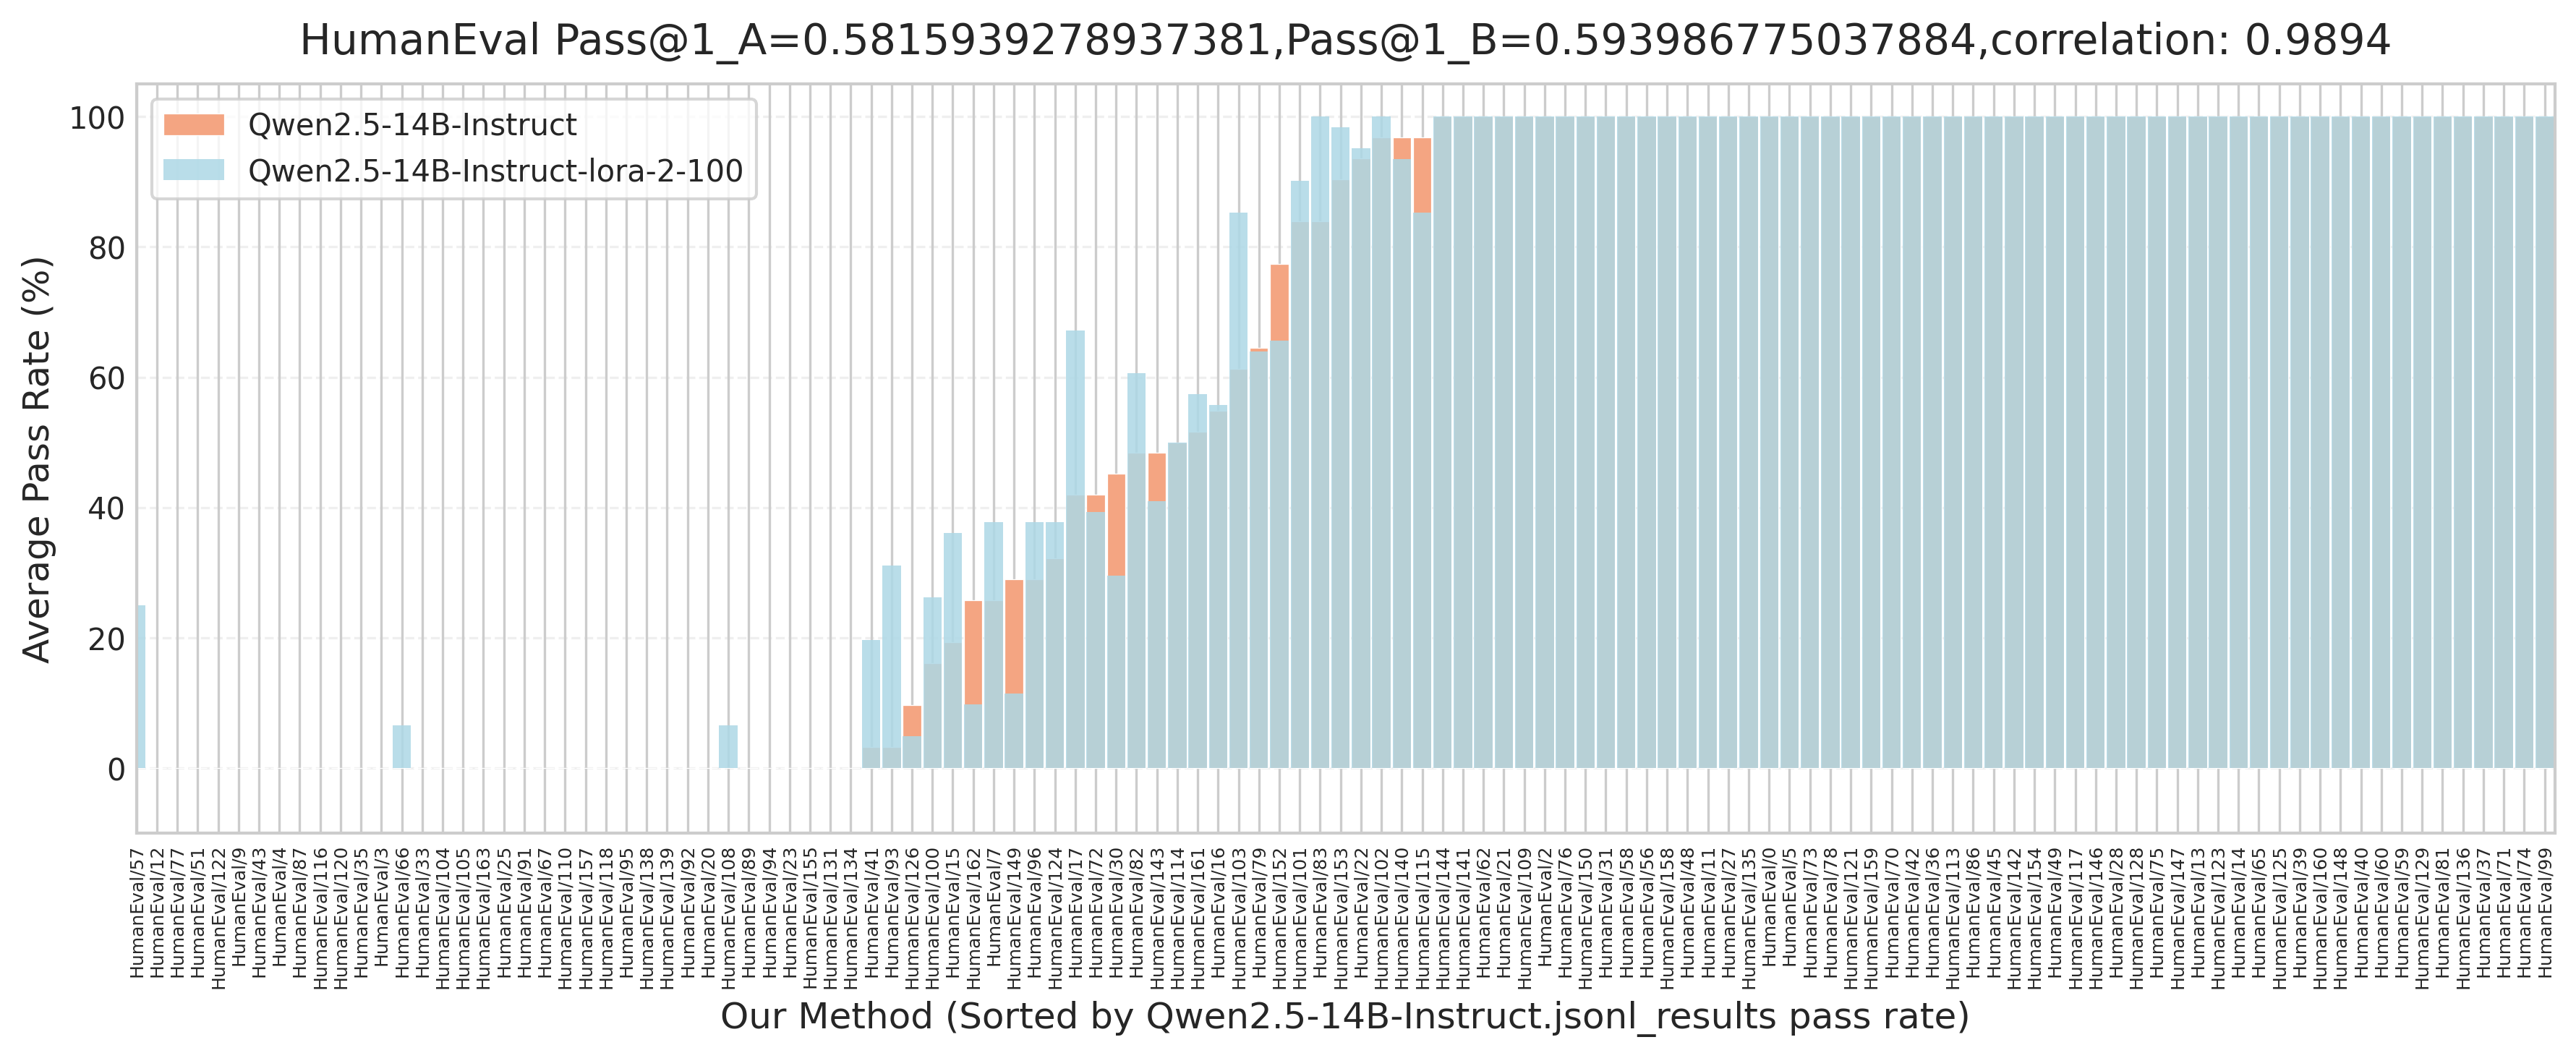
\includegraphics[width=\textwidth]{figures/Qwen2.png}
        \caption{Pass@1 for Qwen2.5-14B on \tool}
        \label{fig:qwensub2}
    \end{subfigure}
    
    \vspace{2mm}
    \caption{The detailed results on the base and \tool{}. The result of \tool{} shows a higher correlation between the clean model and the contaminated model, which means our method can evaluate models more cleanly.}
    \Description{Two scatter plots comparing per-task Pass at 1 scores of Qwen2.5-14B on the original HumanEval benchmark and on CodeArena.}
    \label{fig:Qwen1Comparison}
\end{figure*}

\subsection{Holistic Evaluation on Real-World Models}

We conduct a holistic evaluation of current state-of-the-art LLMs. The evaluation setup is as follows.

\myparagraph{Prompts.} We show the prompt templates for the Defender and Attacker in Appendix~\ref{sec:appendix}.

\myparagraph{Baselines.} We compare against popular evaluation benchmarks, including both fixed-metric and model-based metrics. Appendix~\ref{sec:appendix} details their comparisons.

\begin{enumerate}
\item Static datasets with fixed metrics.
\item Static datasets with model-based metrics.
\item Dynamic datasets such as Auto-Arena.
\end{enumerate}

We also evaluate a small model fine-tuned on HumanEval (LLaMA-13B) for comparison.

\myparagraph{Models.} We evaluate 23 state-of-the-art language models spanning a diverse set of architectures. Our benchmark includes frontier proprietary models such as GPT-4o, o4-mini, Gemini-2.5-Pro, and Claude-3.7-Sonnet, as well as open-source families such as Llama, DeepSeek, and Qwen.

\begin{figure}[!htbp]
  \captionsetup{skip=5pt}
  \centering
  
  \begin{subfigure}[b]{0.48\textwidth}
    \centering
    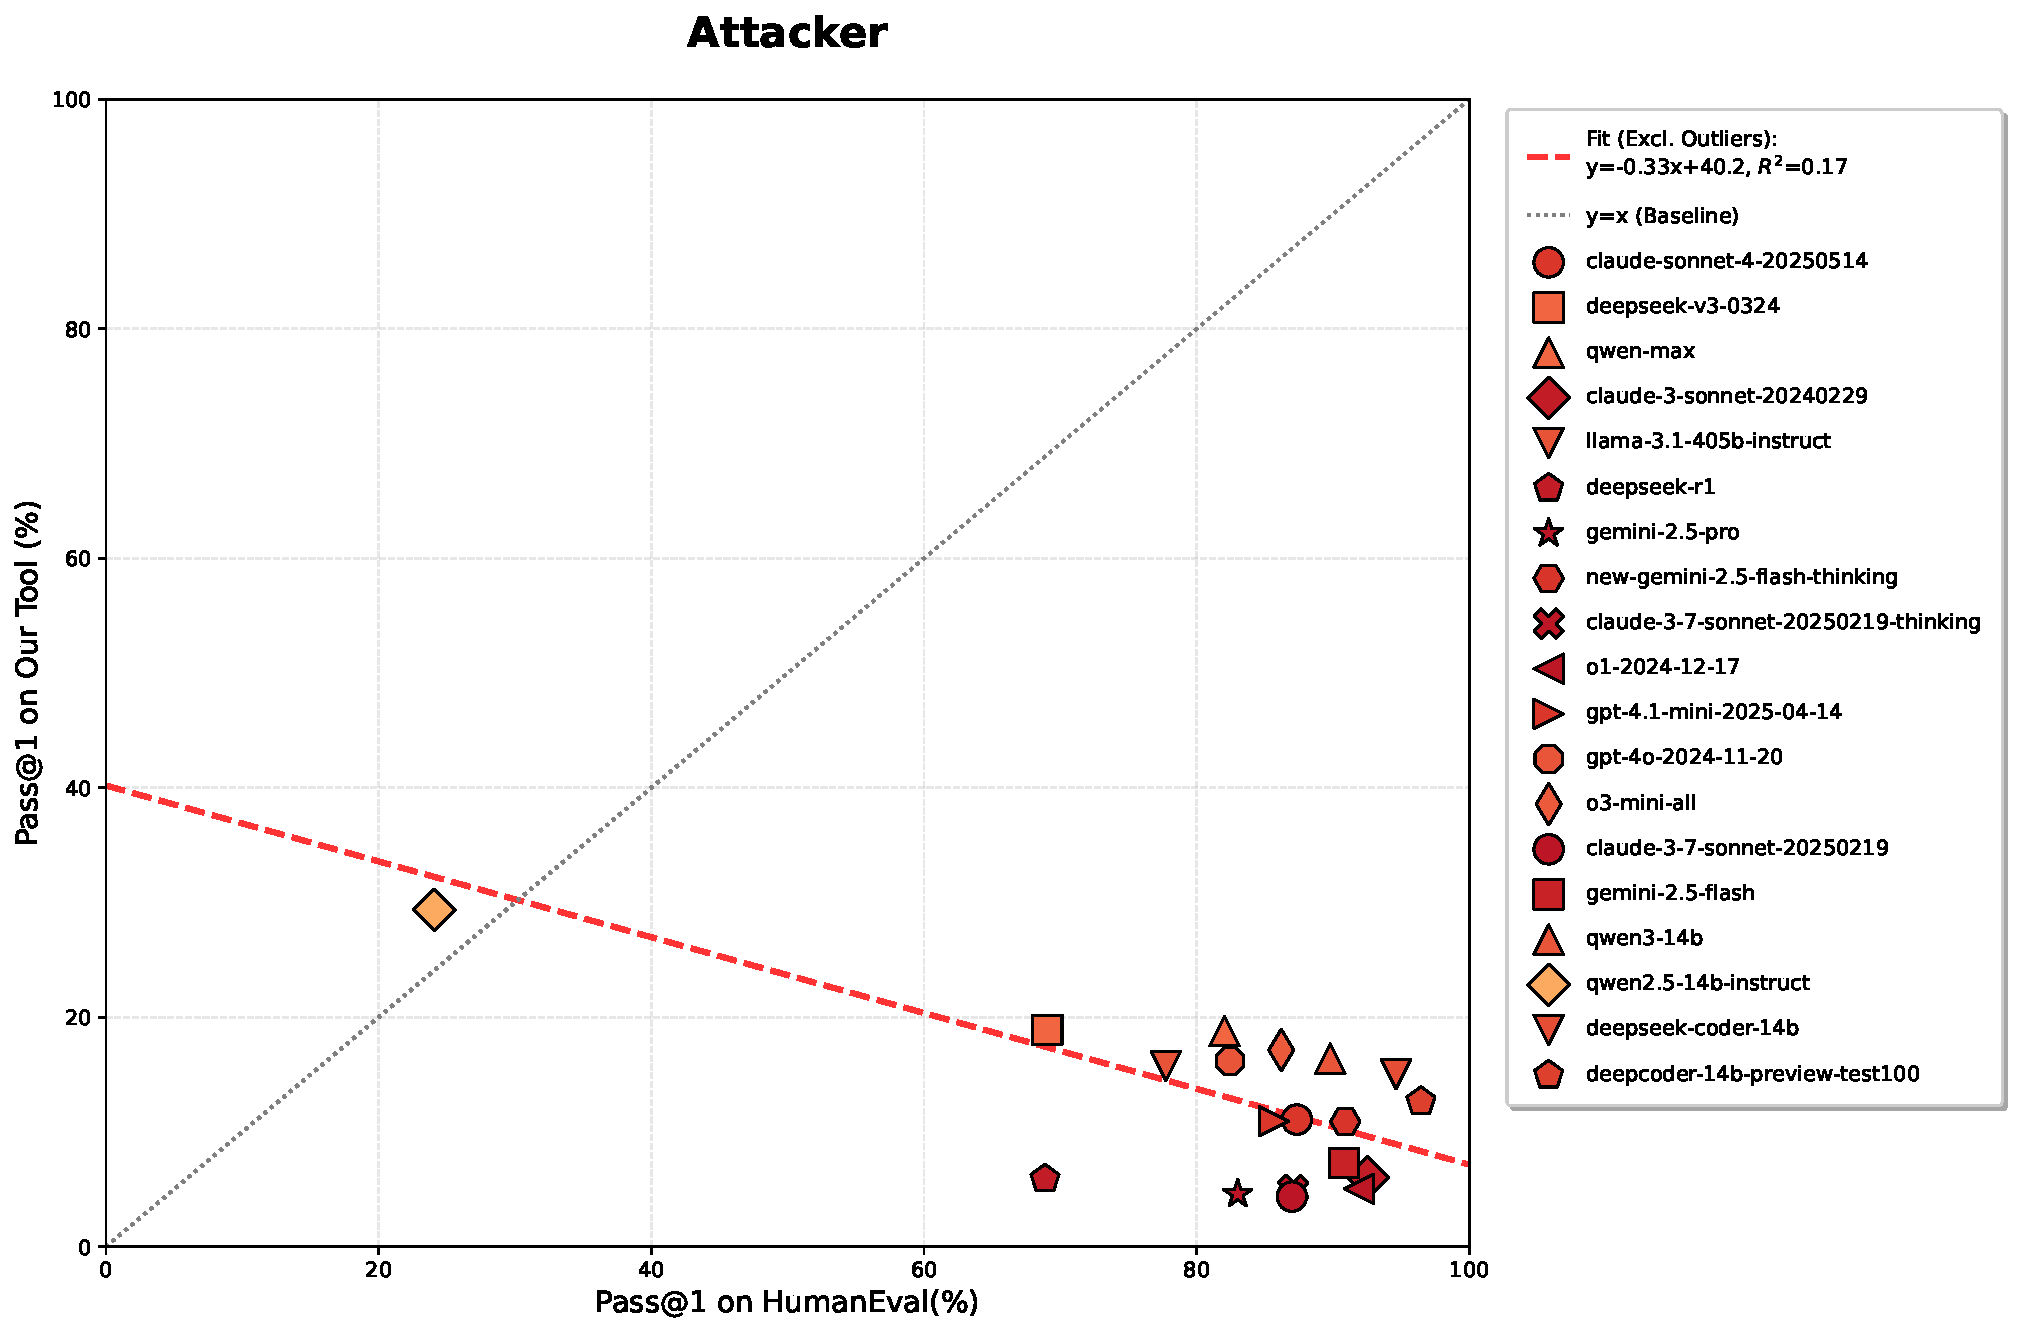
\includegraphics[width=\textwidth]{figures/attacker-weighted-fixed.pdf}
    \caption{Attacker workflow}
    \label{fig:attScore}
  \end{subfigure}
  \hfill
  \begin{subfigure}[b]{0.48\textwidth}
    \centering
    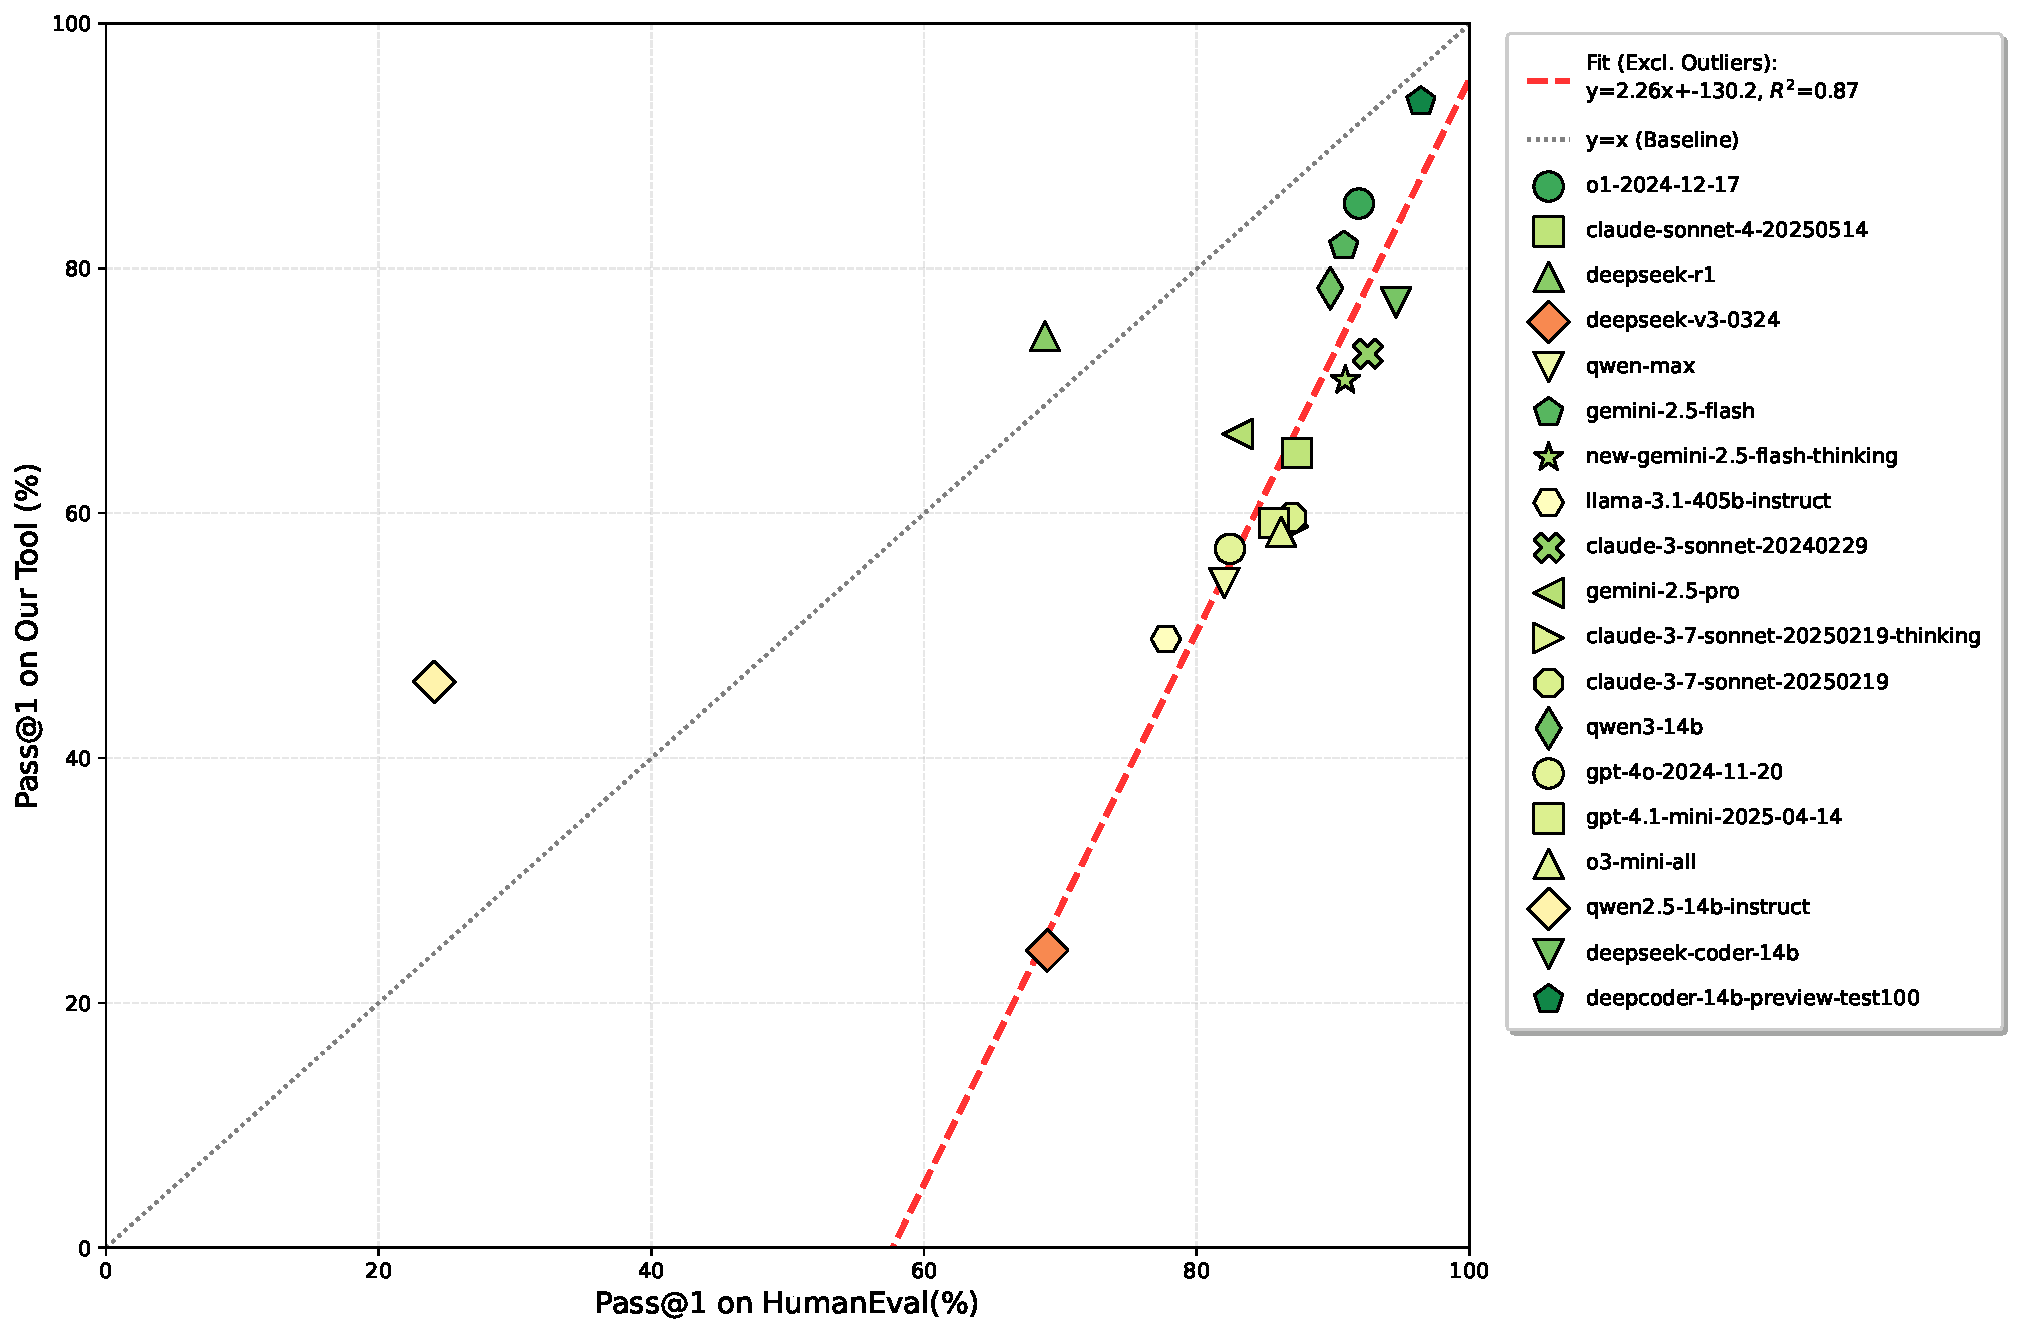
\includegraphics[width=\textwidth]{figures/defenderweightedfixed.pdf}
    \caption{Defender workflow}
    \label{fig:defScore}
  \end{subfigure}
  
  \caption{\tool's workflow: attacker vs defender perspective}
  \Description{Two diagrams side by side illustrating the attacker workflow and the defender workflow in the CodeArena framework.}
  \label{fig:Score}
\end{figure}


% \begin{figure}[!htbp]
% 	% \captionsetup{skip=5pt}
% 	% \centering
% 	% 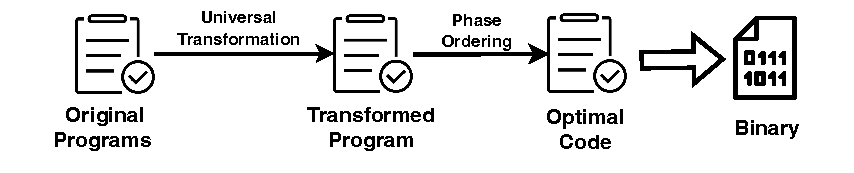
\includegraphics[width=\textwidth]{pics/workflow.pdf}
% 	% \caption{\tool's workflow.}
% 	% \label{fig:keycom}
% \end{figure}






\begin{findingbox}{1}
New tasks generated by models can mitigate data-leakage issues, and models with lower performance may exhibit more pronounced data-leakage problems.
\end{findingbox}

\begin{findingbox}{2}
A model's ability to generate questions has little to do with its ability to perform specific tasks; in fact, there are some models for which the two abilities are completely at odds.
\end{findingbox}

\begin{findingbox}{3}
The performance of LLMs across our variant tasks and the original tasks exhibits a high level of linear correlation, but with larger variance, thereby narrowing the gap between models.
\end{findingbox}

% \begin{figure*}[t!]
%     \centering
%     % --- 第一张子图 ---
%     \begin{subfigure}[b]{0.48\textwidth}
%         \centering
%         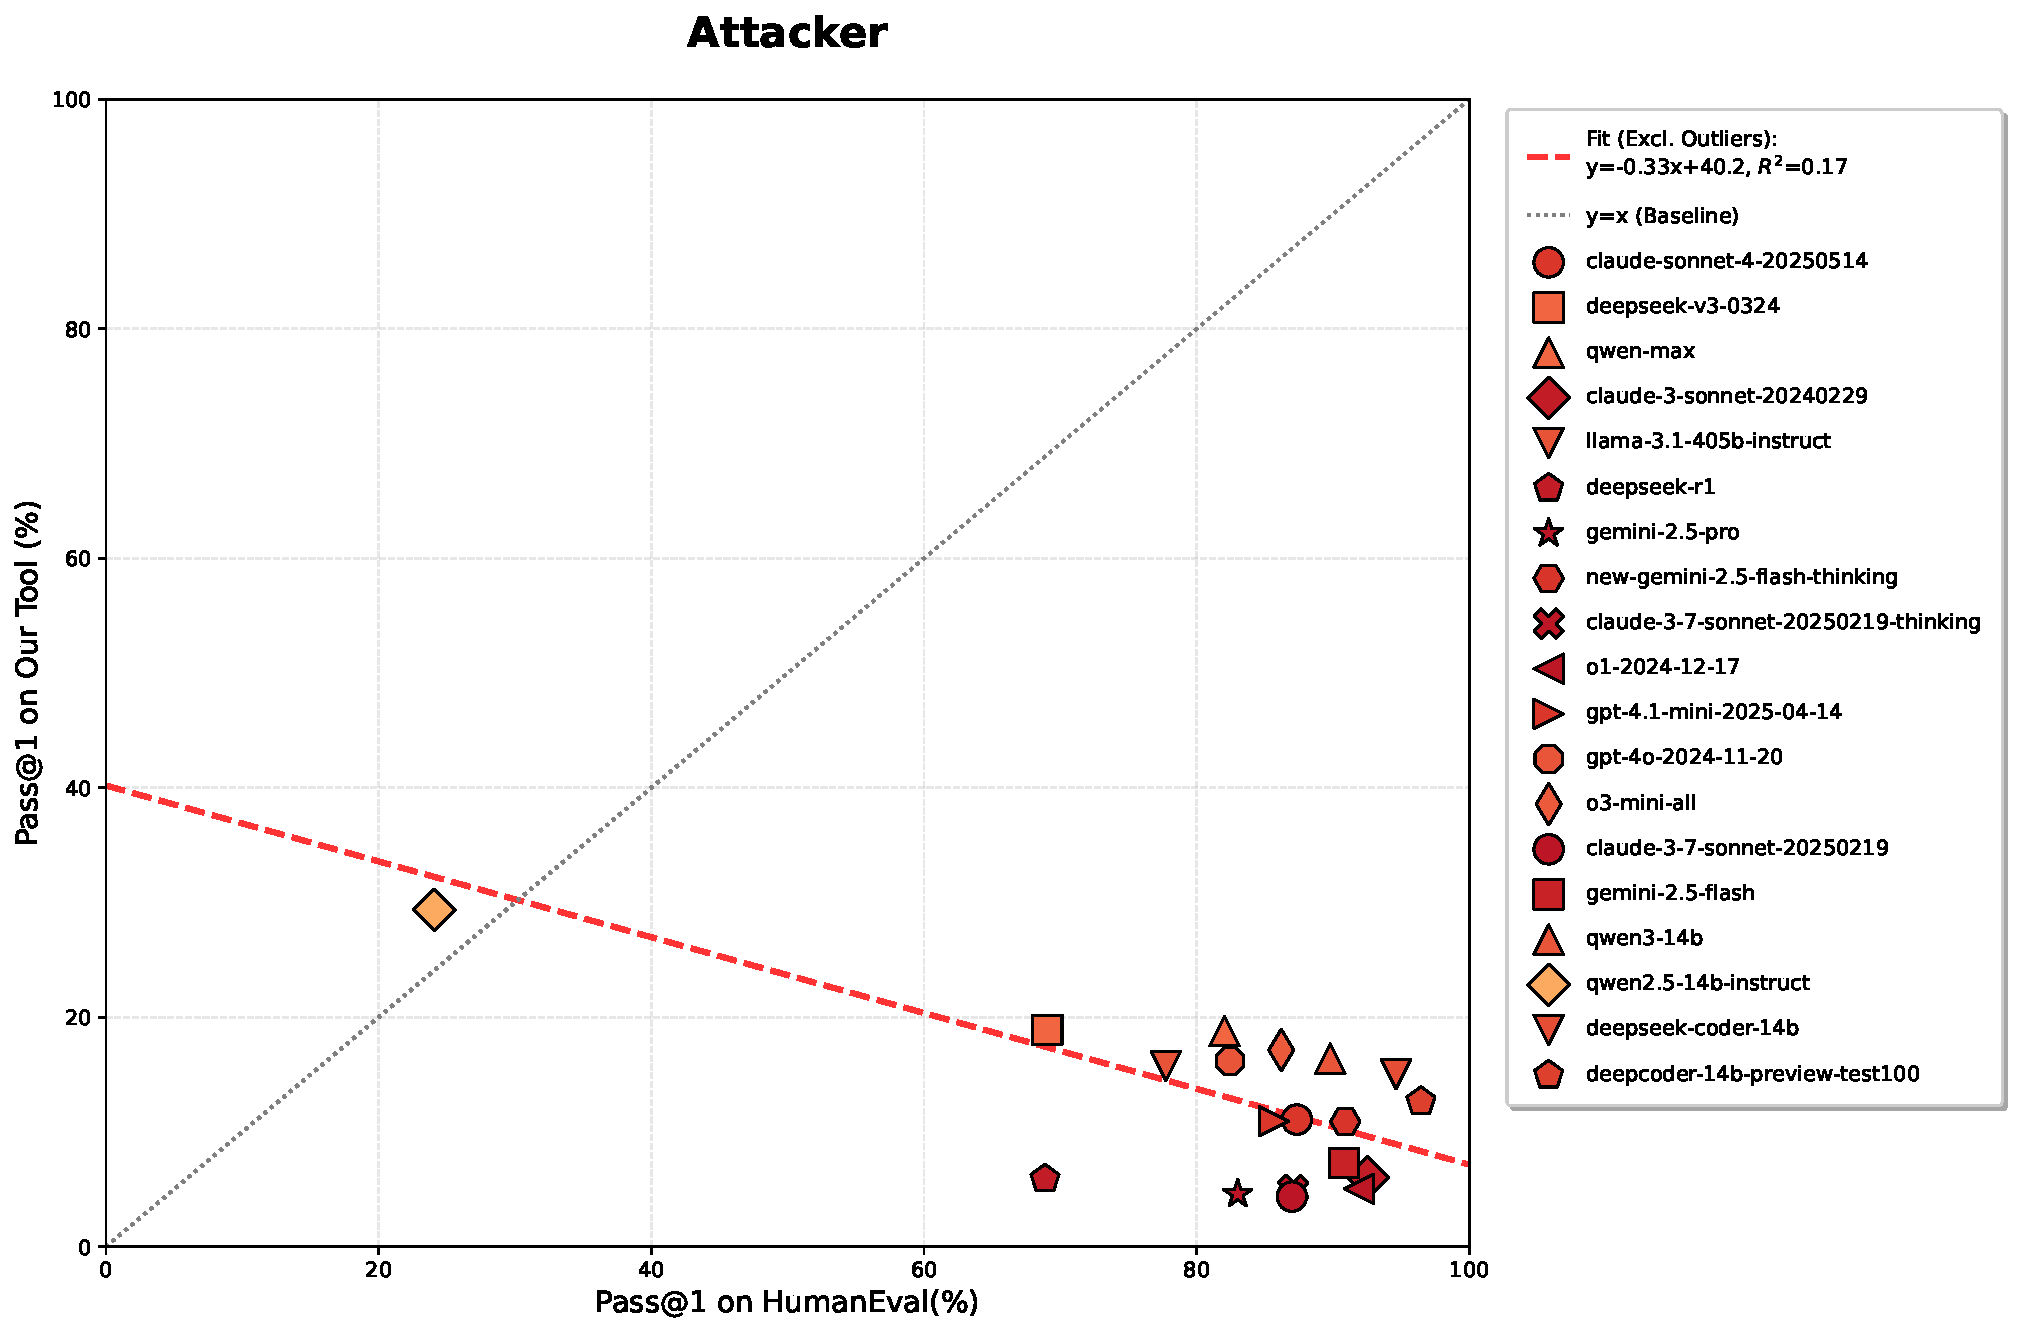
\includegraphics[width=\textwidth]{figures/attacker-weighted-fixed.pdf}
%         \caption{Attacker perspective}
%         \label{fig:exp2_def_attacker}
%     \end{subfigure}
%     \hfill
%     % --- 第二张子图 ---
%     \begin{subfigure}[b]{0.48\textwidth}
%         \centering
%         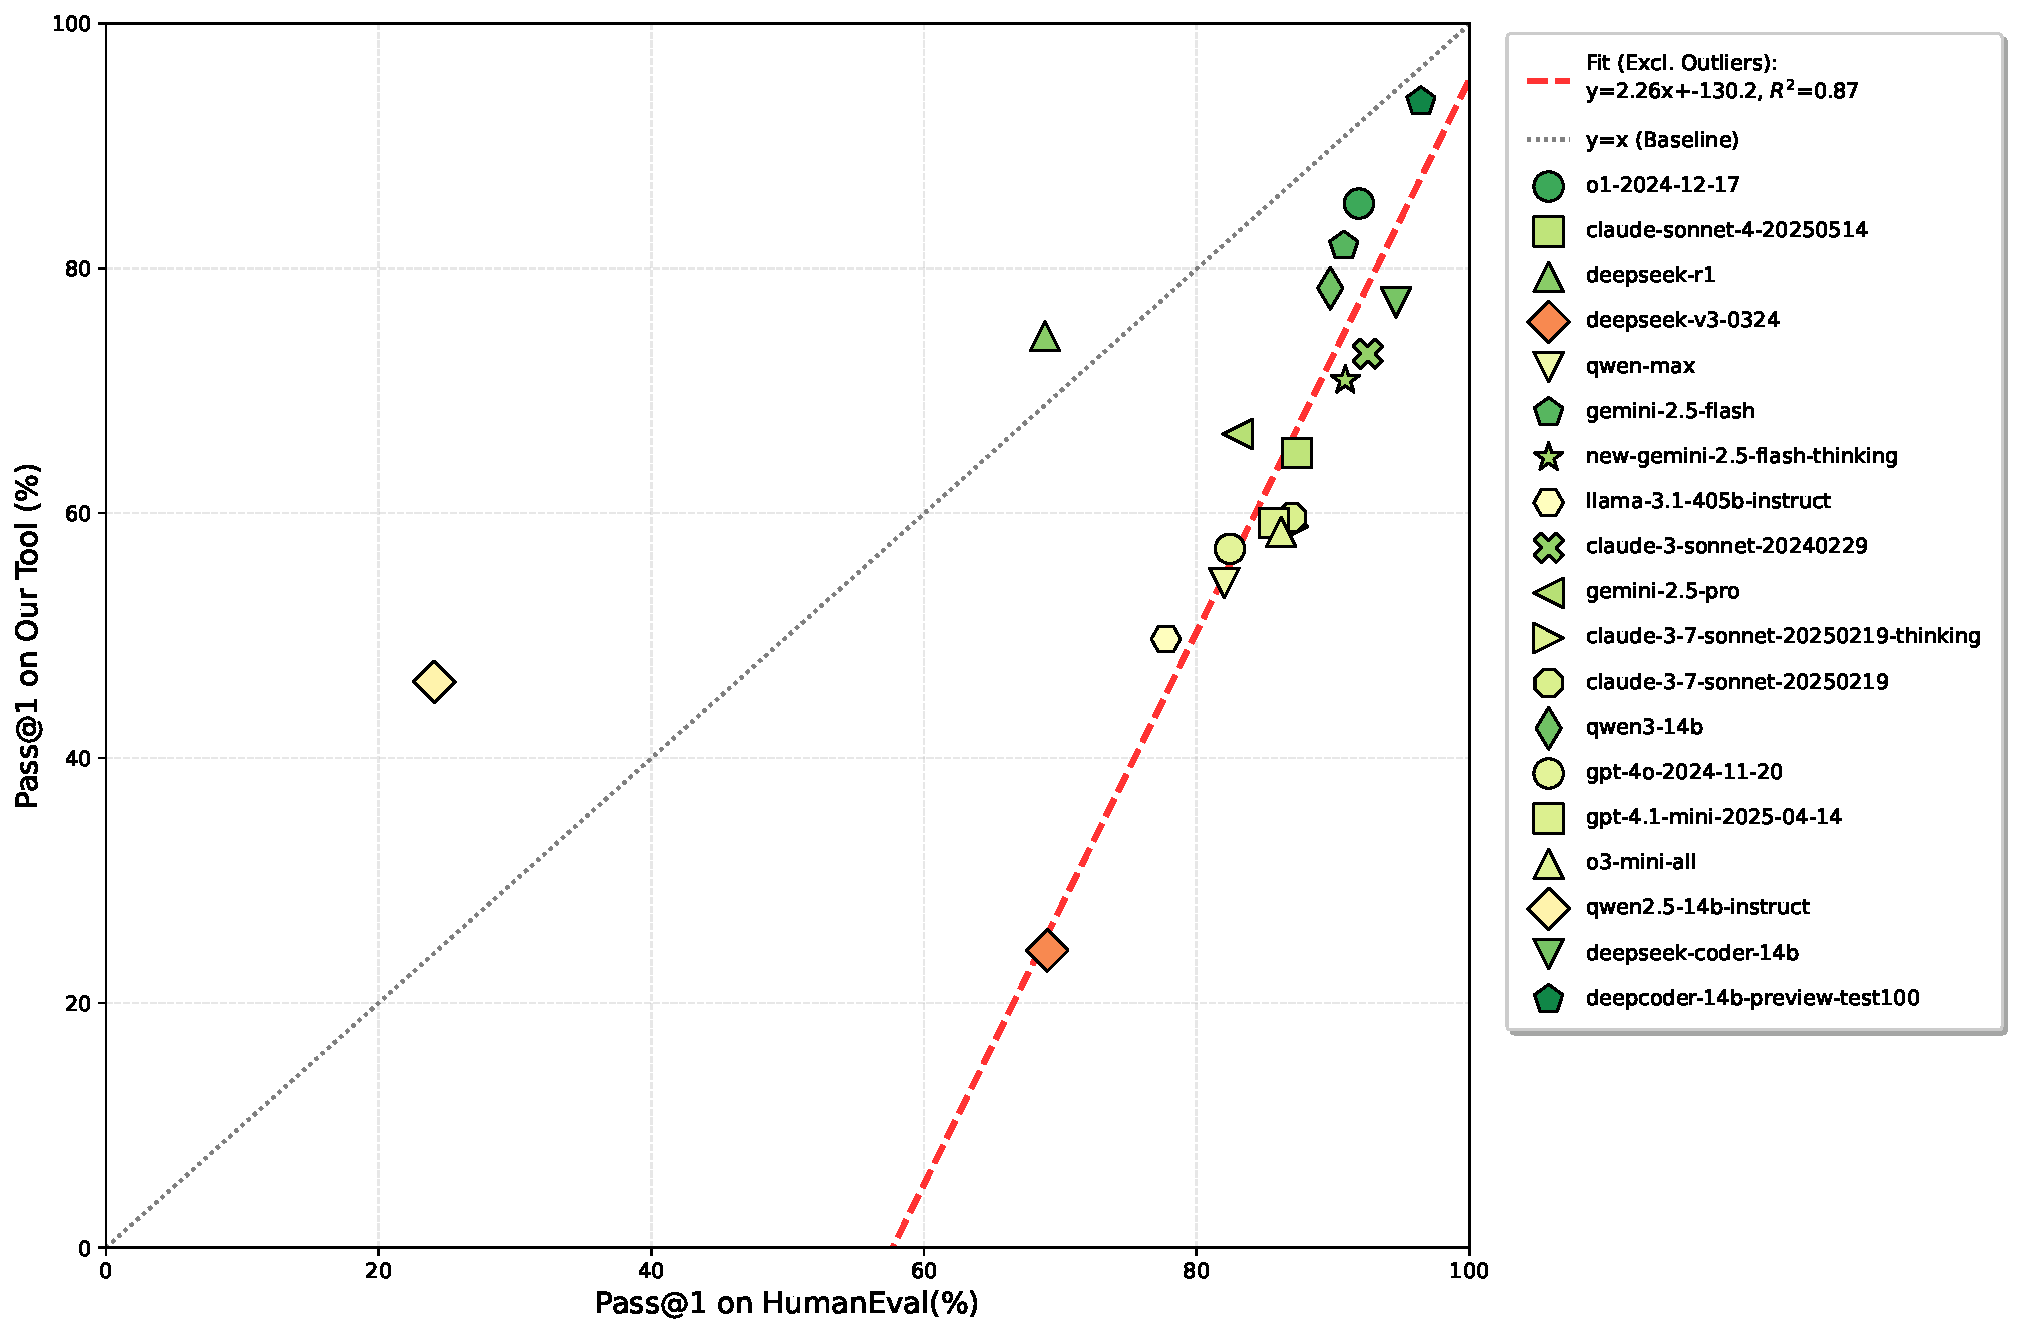
\includegraphics[width=\textwidth]{figures/defenderweightedfixed.pdf}
%         \caption{Defender perspective}
%         \label{fig:exp2_def_defender}
%     \end{subfigure}

%     \vspace{4mm}
%     \caption{\tool{} vs HumanEval: comparison from both perspectives. The results show the performance difference between attacker and defender workflows.}
%     \label{fig:exp2_def}
% \end{figure*}



\begin{figure}[!htbp]
  \captionsetup{skip=5pt}
  \centering
  
  \begin{subfigure}[b]{0.48\textwidth}
    \centering
    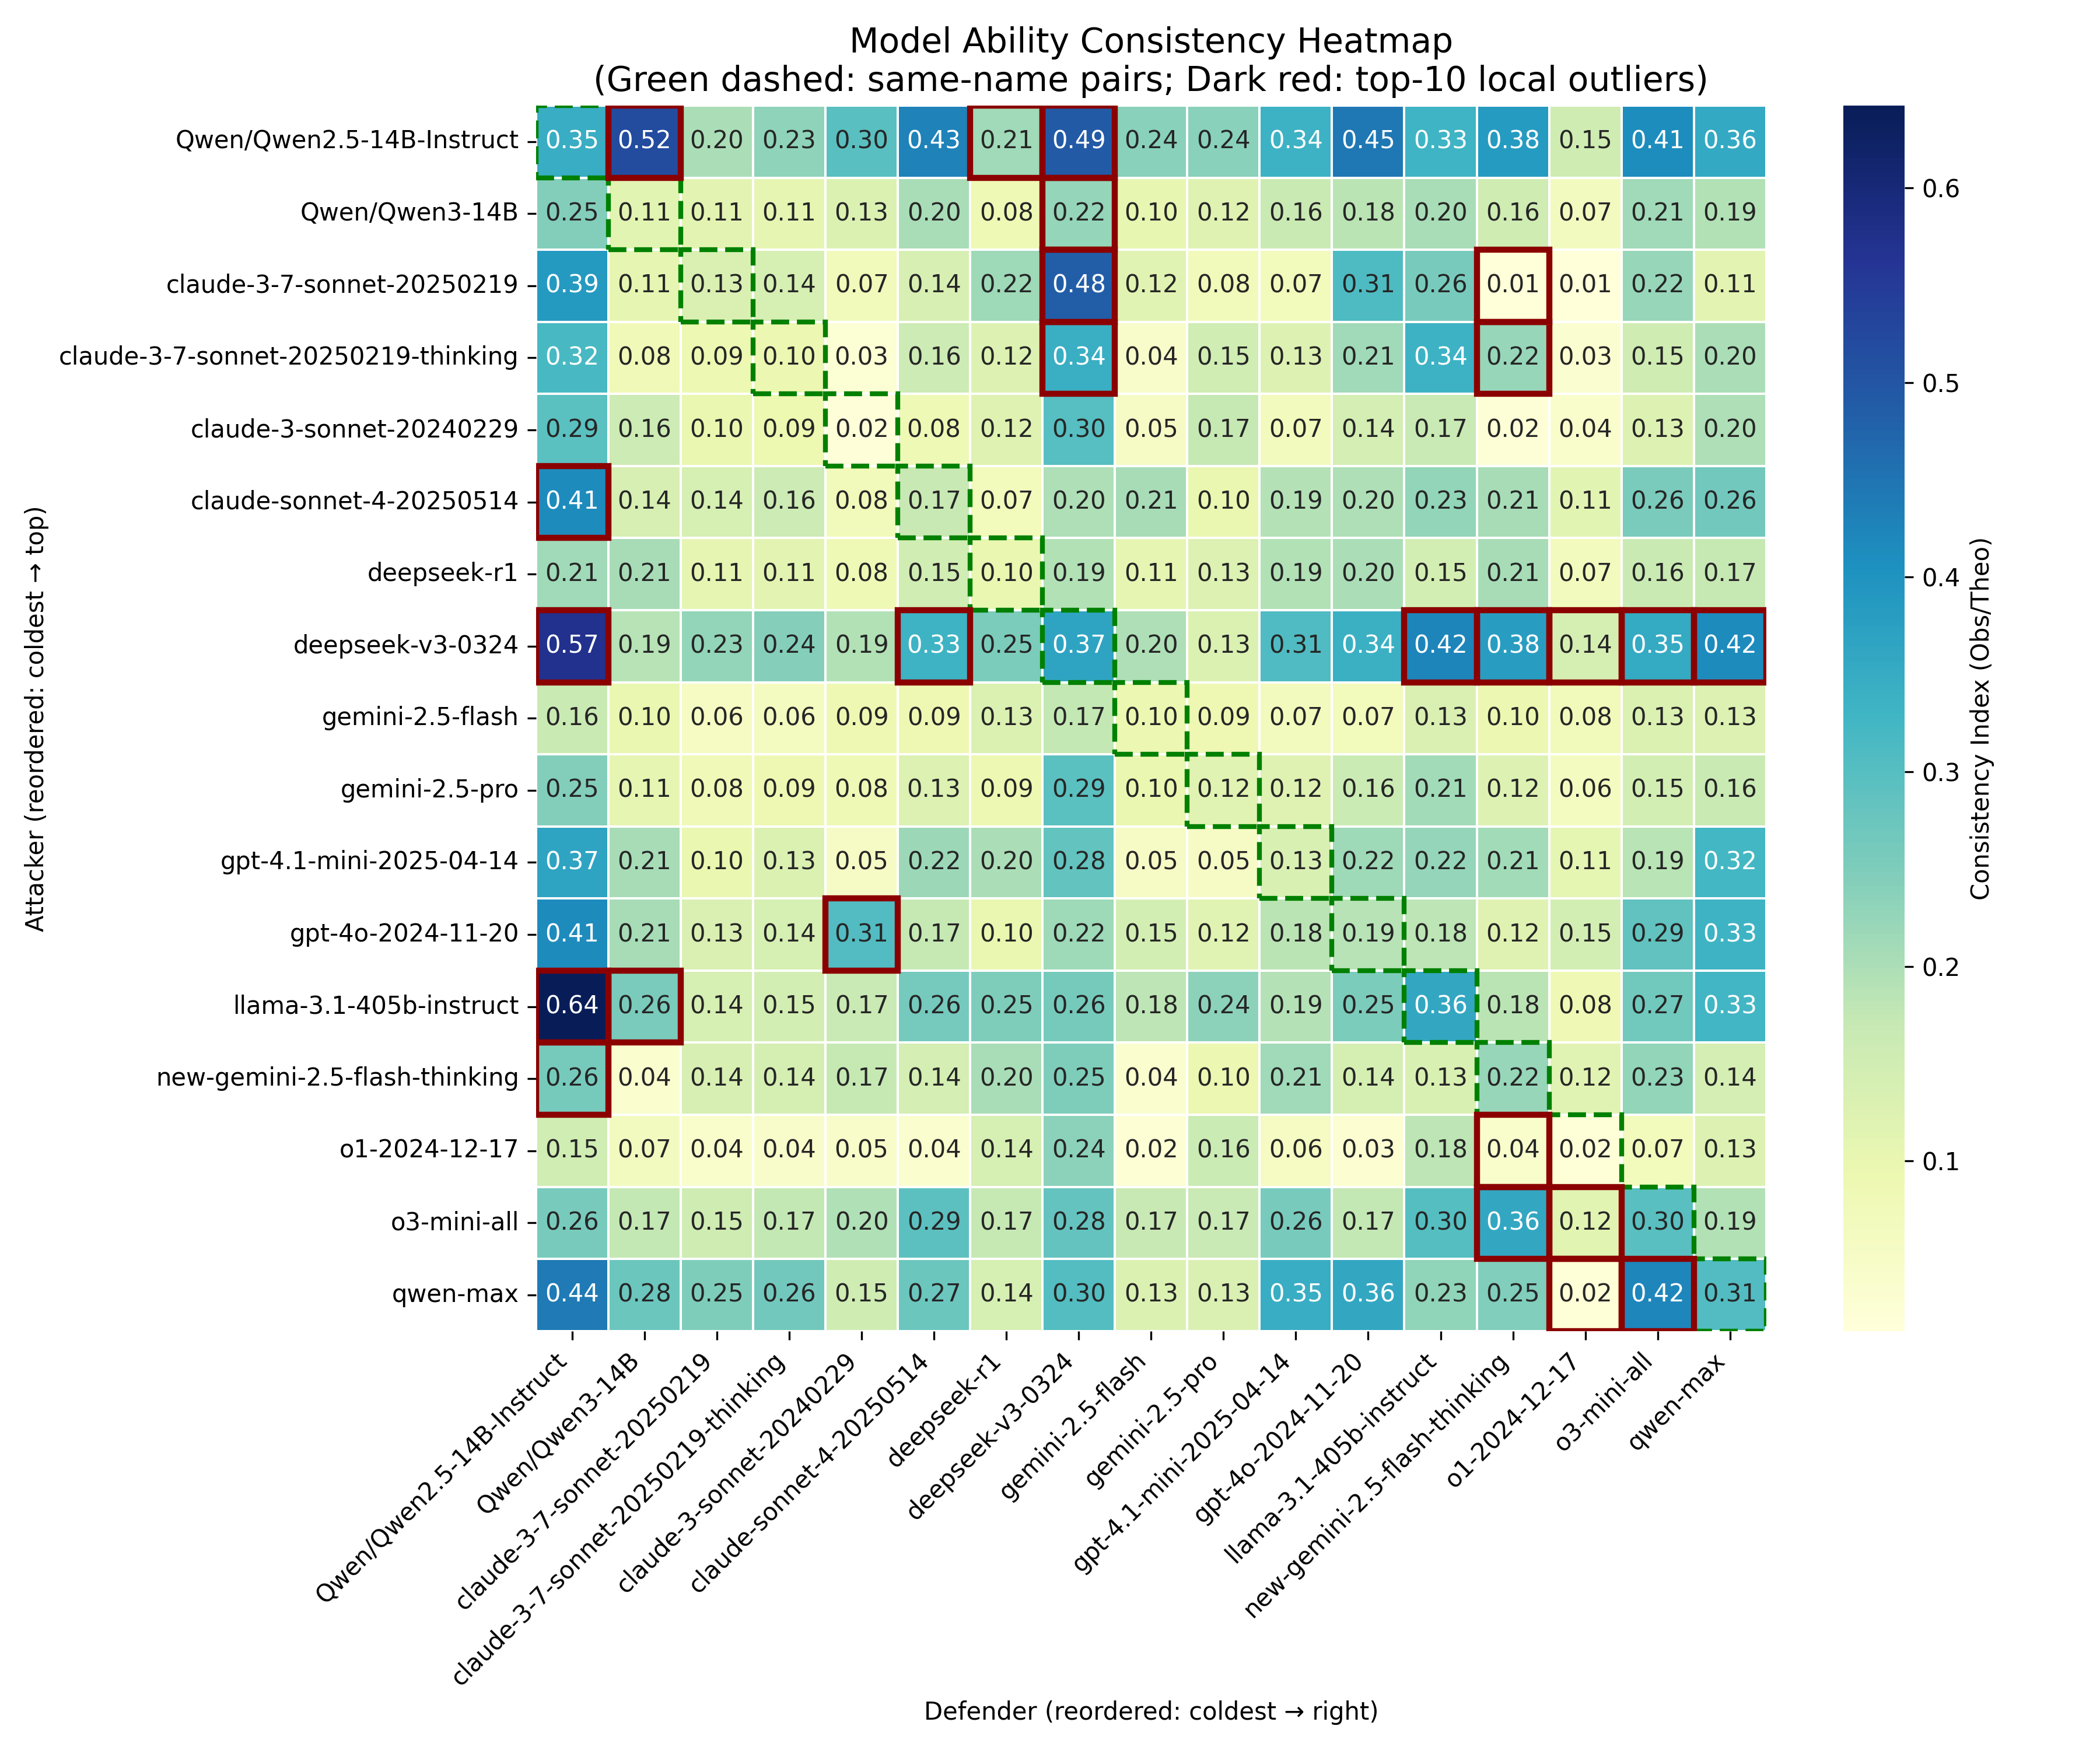
\includegraphics[width=\textwidth]{figures/styleconsistencyheatmaporiginal.png}
    \caption{Attacker workflow}
    \label{fig:figattattacker}
  \end{subfigure}
  \hfill
  \begin{subfigure}[b]{0.48\textwidth}
    \centering
    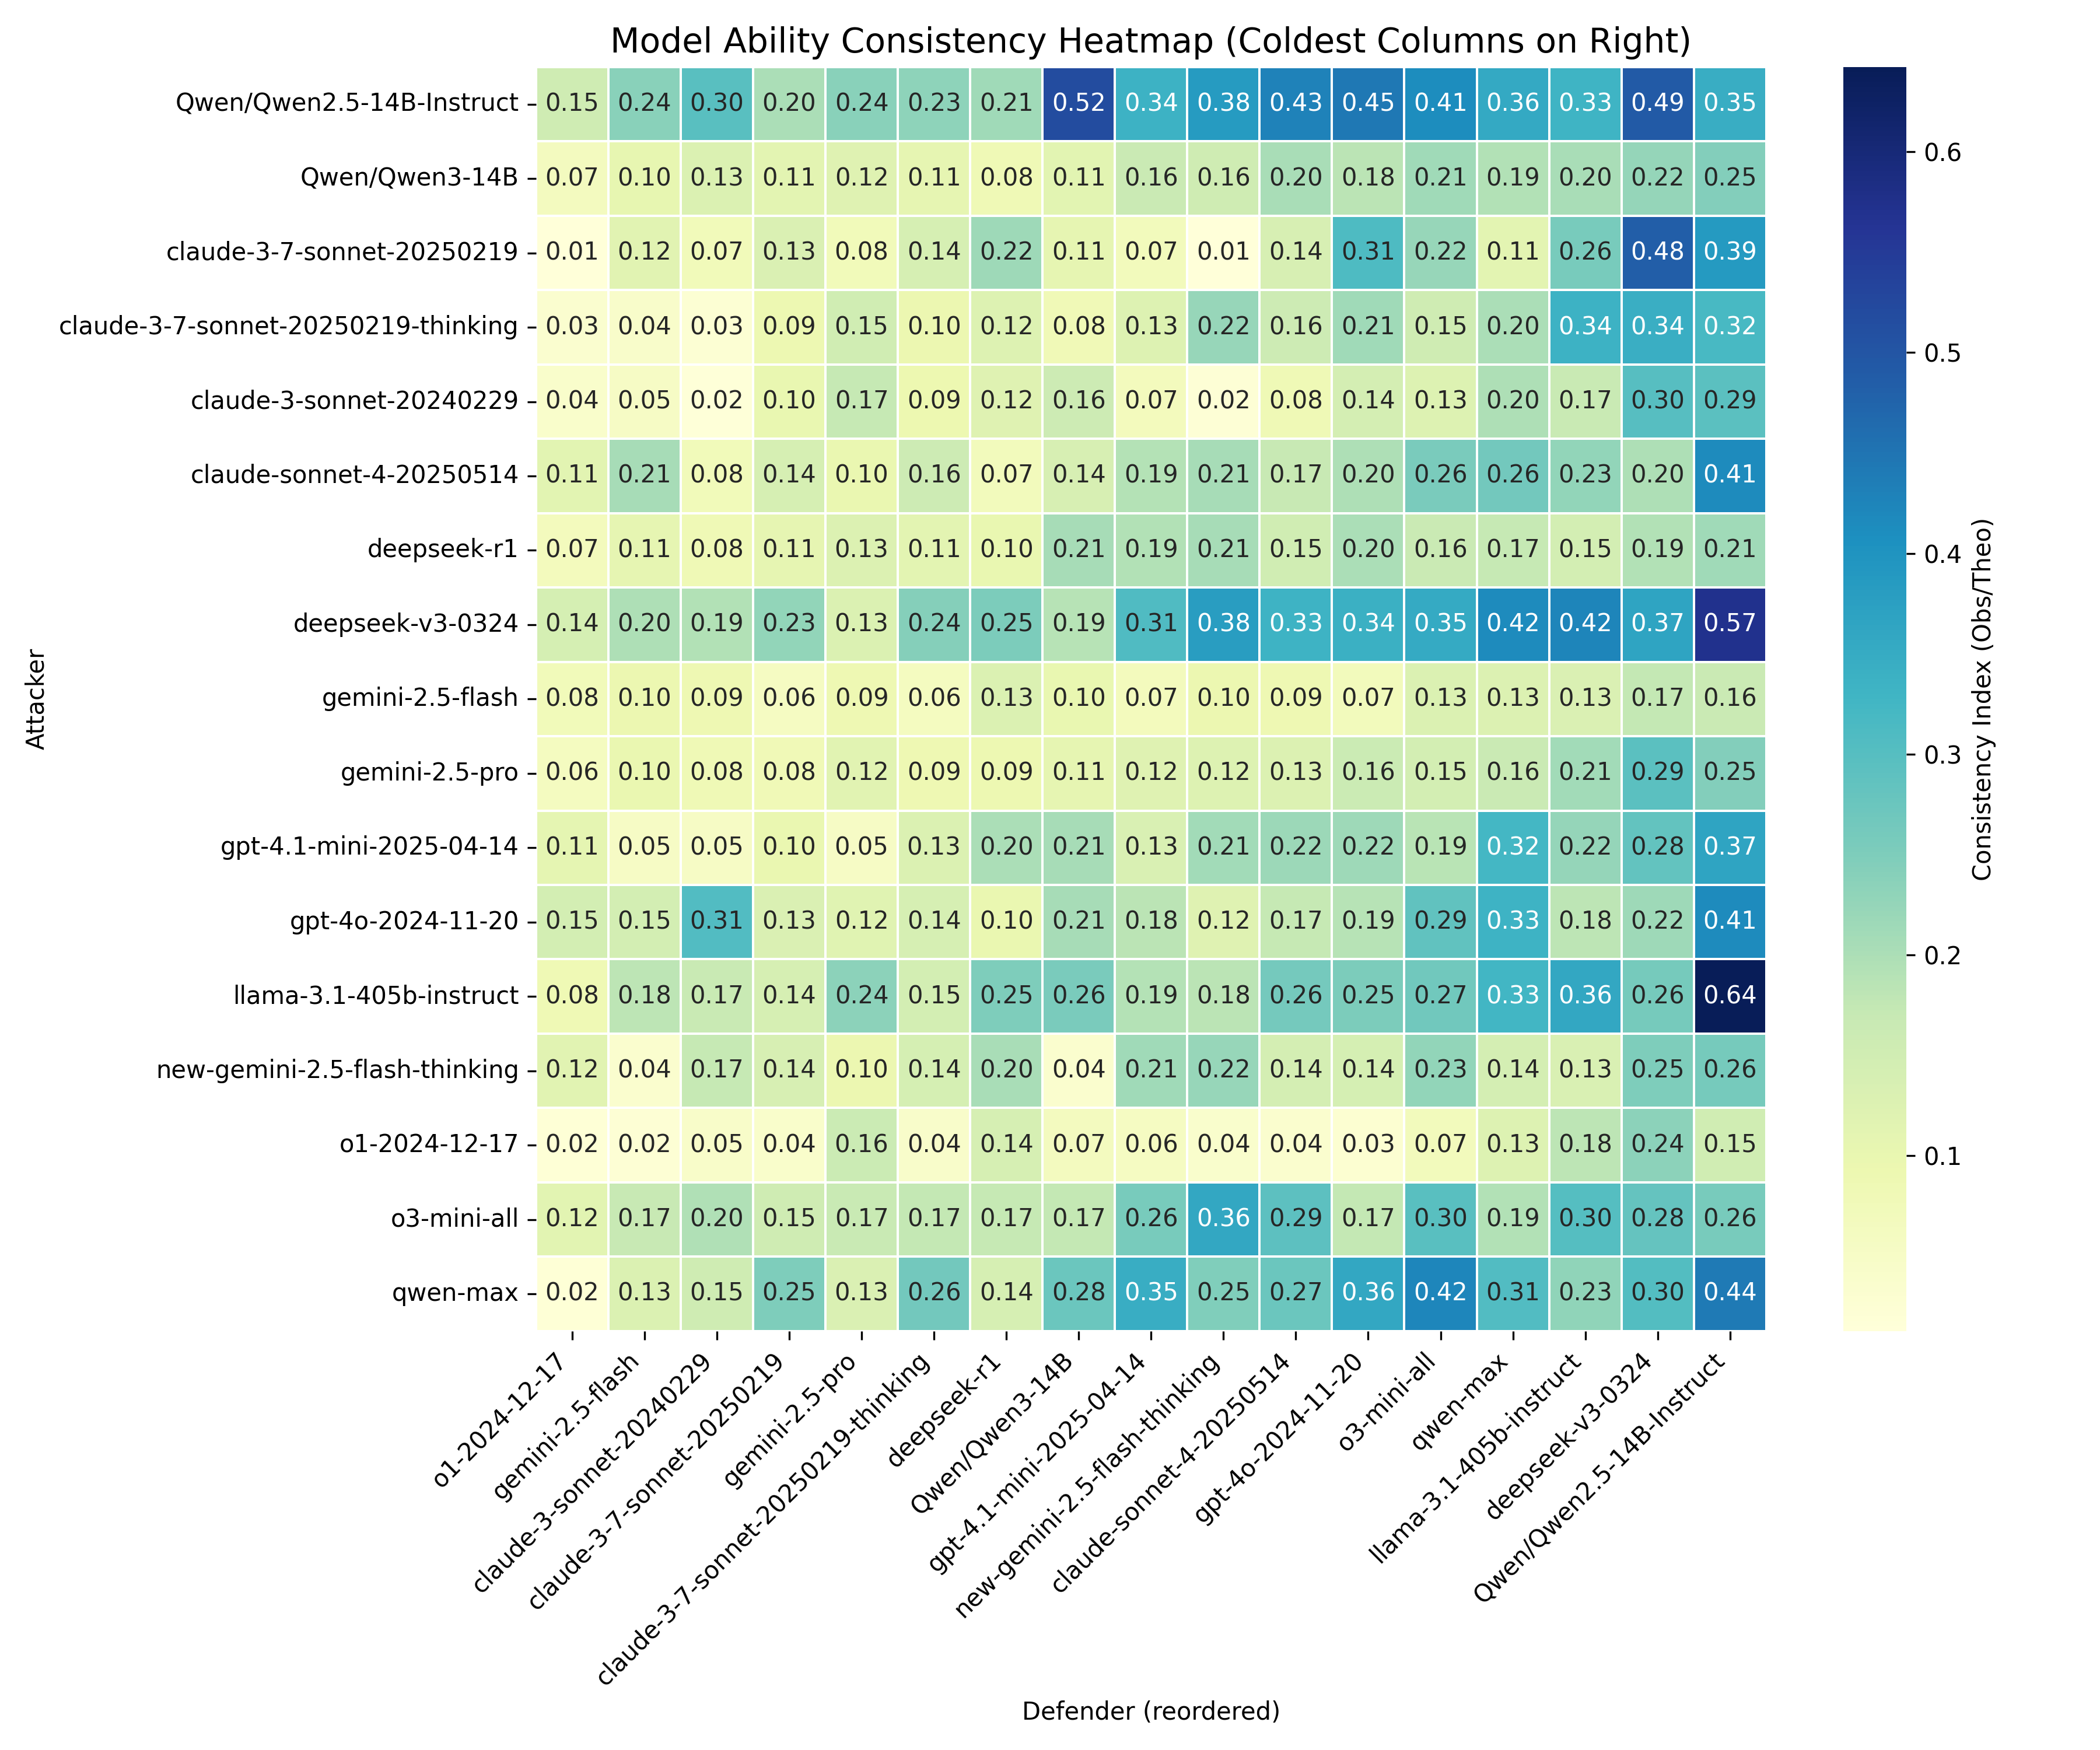
\includegraphics[width=\textwidth]{figures/styleconsistencyheatmap222.png}
    \caption{Defender workflow}
    \label{fig:figattdefender}
  \end{subfigure}
  
  \caption{\tool's workflow: attacker vs defender perspective}
  \Description{Two heatmaps comparing style consistency from the attacker perspective and the defender perspective.}
  \label{fig:figatt}
\end{figure}

We identify a significant divergence between humans and LLMs in their judgment of problem difficulty. Further analysis is provided in the discussion section.

\myparagraph{Metric: unPass@$k$.} In addition to standard Pass@$k$, we introduce unPass@$k$ as a normalized metric that accounts for the difficulty of the attacking tasks.

\subsection{Cost Comparison}

We use consumed tokens to represent cost. The results show that our method's consumption is both economical and affordable for individuals. A detailed cost analysis is included in Appendix~\ref{sec:appendix}.

\subsection{Ablation Studies on Seed Problems}

We conduct ablation studies to understand the influence of seed-problem selection on the quality of generated mutations. Preliminary results indicate that selecting problems with moderate initial difficulty yields the most discriminative mutated tasks. We leave a full analysis to the final version of the paper.


\bibliographystyle{ACM-Reference-Format}
\bibliography{reference}

\appendix
\section{Appendix}
\label{sec:appendix}

Prompts, baseline descriptions, and a detailed cost analysis are provided in the final version of the paper.

\end{document}
